% Déclaration du type de document (report, book, paper, etc...)
\documentclass[a4paper, 12pt]{paper} 
 
% Package pour avoir Latex en français
\usepackage[utf8]{inputenc}
\usepackage[T1]{fontenc}
 
% Quelques packages utiles
\usepackage{listings} % Pour afficher des listings de programmes
\usepackage{graphicx} % Pour afficher des figures
\usepackage{amsthm}   % Pour créer des théorèmes et des définitions
\usepackage{amsmath}
\usepackage{microtype} % Optical margins FTW
\usepackage{url}
\usepackage{booktabs} % Allows the use of \toprule, \midrule and \bottomrule in tables for horizontal lines
\usepackage[per-mode=symbol]{siunitx}
\usepackage{floatrow}
\usepackage{caption}
\usepackage{subcaption}
\usepackage{fullpage}
\usepackage{lipsum}



\author{Loïc Amez-Droz \and Florian Reinhard}
\title{Detector and Noise}

% Début du document
\begin{document}
\begin{titlepage}
\begin{center}
    \textsc{\LARGE École Polytechnique Fédérale de~Lausanne}\\[1.5cm] 
    {\huge \bfseries Optical Engineering: Multimode Fibre}\\[0.4cm] 
    \begin{tabular}{|p{5cm}|p{4cm}|}
        \hline
        Group & C-XX \\ \hline
        Students & Loïc \textsc{Amez-Droz} \newline Florian \textsc{Reinhard} \\ \hline
        Date of lecture & 13.03.2015 \\ \hline
        Date of final report return & 20.03.2015 \\ \hline
    \end{tabular}
\end{center}


\begin{abstract}
    \lipsum[3]
\end{abstract}
 
\vfill
\end{titlepage}

\section{Procedures and results}
\subsection{Noise evaluation}

We evaluate the impact of different exposure times and gain levels on the noise.


\begin{table}[H]
    \centering
    \begin{tabular}{l S[table-format=3.3] S[table-format=1.3] S[table-format=3.3] S[table-format=1.3] S[table-format=3.3] S[table-format=1.3]}
        \toprule
        Conditions & {$\mu_R$} & {$\sigma_R$} & {$\mu_G$} & {$\sigma_G$} & {$\mu_B$} & {$\sigma_B$} \\
        \midrule
        w/o light, max exposure, max gain & 4.166 & 2.558 & 4.196 & 2.308 & 2.651 & 2.114\\
        w/o light, min exposure, min gain & 1.724 & 0.430 & 1.876 & 0.490 & 1.759 & 0.442 \\
        w/o light, max exposure, min gain & 1.528 & 0.516 & 1.912 & 0.684 & 1.623 & 0.566 \\
        w/o light, min exposure, max gain & 2.696 & 1.689 & 3.183 & 1.630 & 1.694 & 1.468 \\
        nearly saturated, max gain & 199.316 & 5.567 & 184.123 & 7.396 & 179.742 & 6.386 \\
        nearly saturated, min gain & 216.254 & 3.307 & 205.610 & 6.538 & 199.274 & 5.022 \\
        \bottomrule
    \end{tabular}
    \caption{Mean $\mu$ and standard deviation $\sigma$ of all three color channels of pictures with different conditions.}
\label{tab:means_stds}
\end{table}

% Channel: blue

\begin{figure}[H]
    \centering
    \begin{subfigure}[b]{0.45\textwidth}
        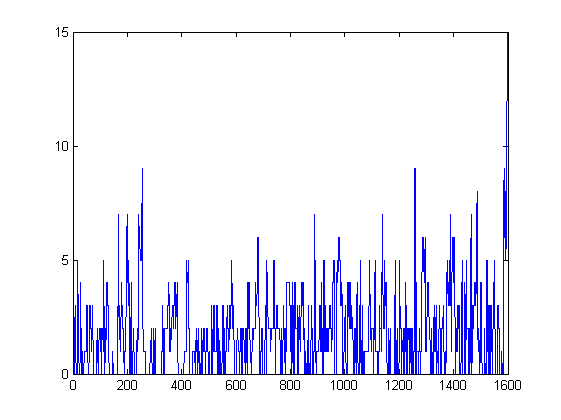
\includegraphics[width=\textwidth]{img/plot_black_a}
        \caption{Max exposure, max gain.}
    \end{subfigure}
    \begin{subfigure}[b]{0.45\textwidth}
        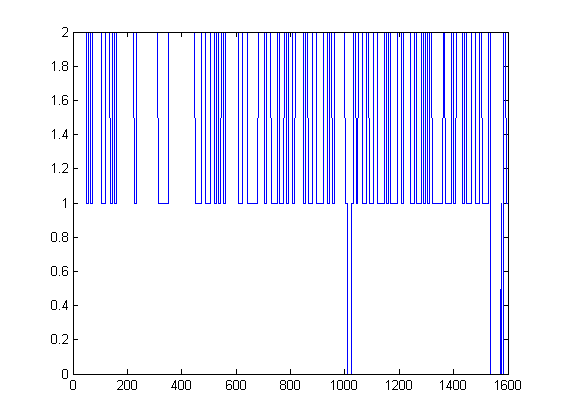
\includegraphics[width=\textwidth]{img/plot_black_b}
        \caption{Min exposure, min gain.}
    \end{subfigure}
    \begin{subfigure}[b]{0.45\textwidth}
        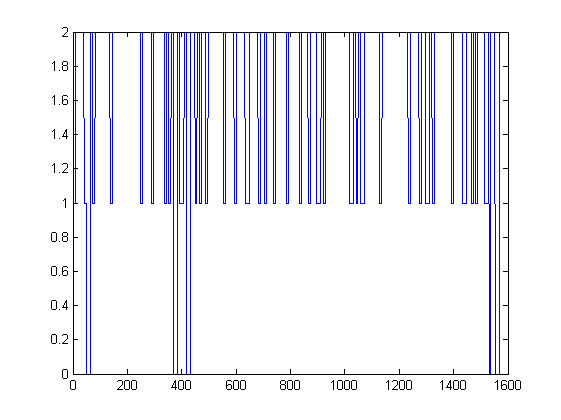
\includegraphics[width=\textwidth]{img/plot_black_c}
        \caption{Max exposure, min gain.}
    \end{subfigure}
    \begin{subfigure}[b]{0.45\textwidth}
        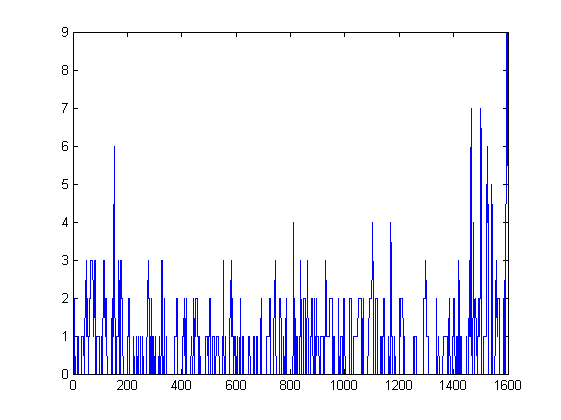
\includegraphics[width=\textwidth]{img/plot_black_d}
        \caption{Min exposure, max gain.}
    \end{subfigure}
    \caption{Line plots of the blue channel of pictures with the light blocked by a black cloth showing the \emph{dark noise}. The \emph{gain} amplifies the dark noise while the exposure time has very little effect.}
\label{fig:black}
\end{figure}

\begin{figure}[H]
    \centering
    \begin{subfigure}[b]{0.45\textwidth}
        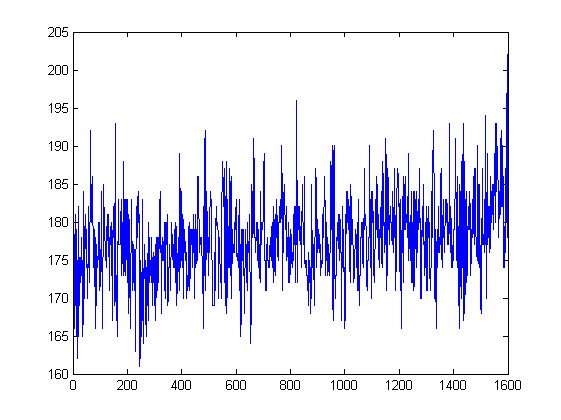
\includegraphics[width=\textwidth]{img/plot_max_gain}
        \caption{Max gain.}
    \end{subfigure}
    \begin{subfigure}[b]{0.45\textwidth}
        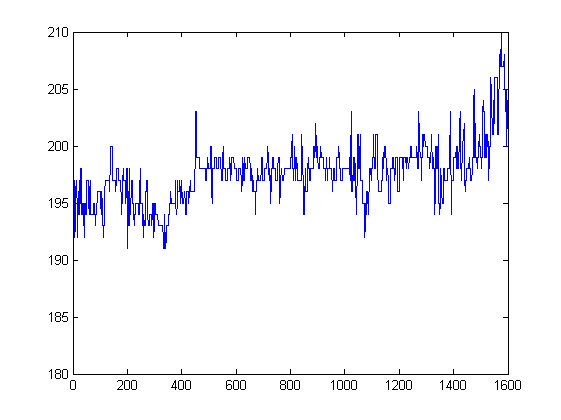
\includegraphics[width=\textwidth]{img/plot_no_gain}
        \caption{Min gain.}
    \end{subfigure}
    \caption{Line plots of the blue channel of pictures with a uniform illumination. Less gain seems to reduce the noise.}
\label{fig:nearly_sat}
\end{figure}

\subsection{Noise reduction by averaging}
% Channel: red
This experiment shows that the noise can be reduced by averaging different lines of the picture.
We compare the noise levels for low and high gains after averaging of one respectively many lines.

\begin{figure}[H]
    \centering
    \begin{subfigure}[b]{0.47\textwidth}
        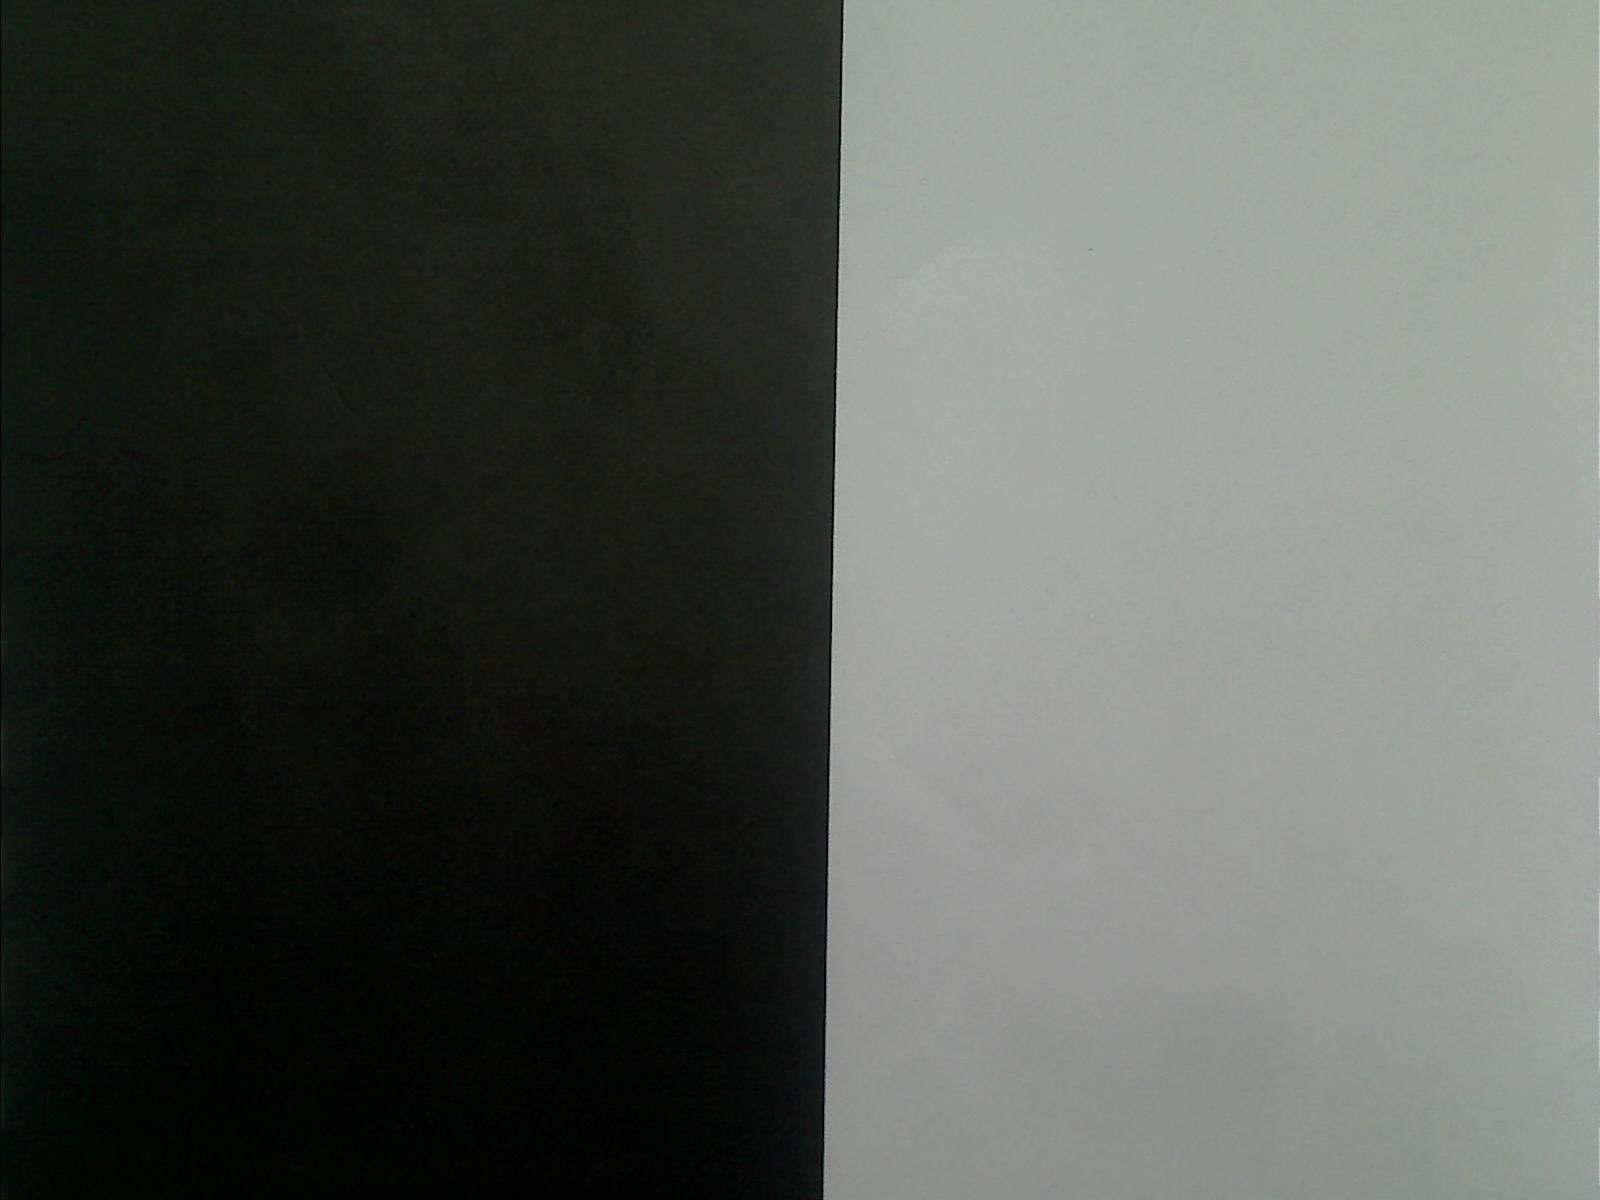
\includegraphics[width=\textwidth]{img/contrast_no_gain.jpg}
        \caption{Photo with low gain.}
    \end{subfigure}
    \begin{subfigure}[b]{0.47\textwidth}
        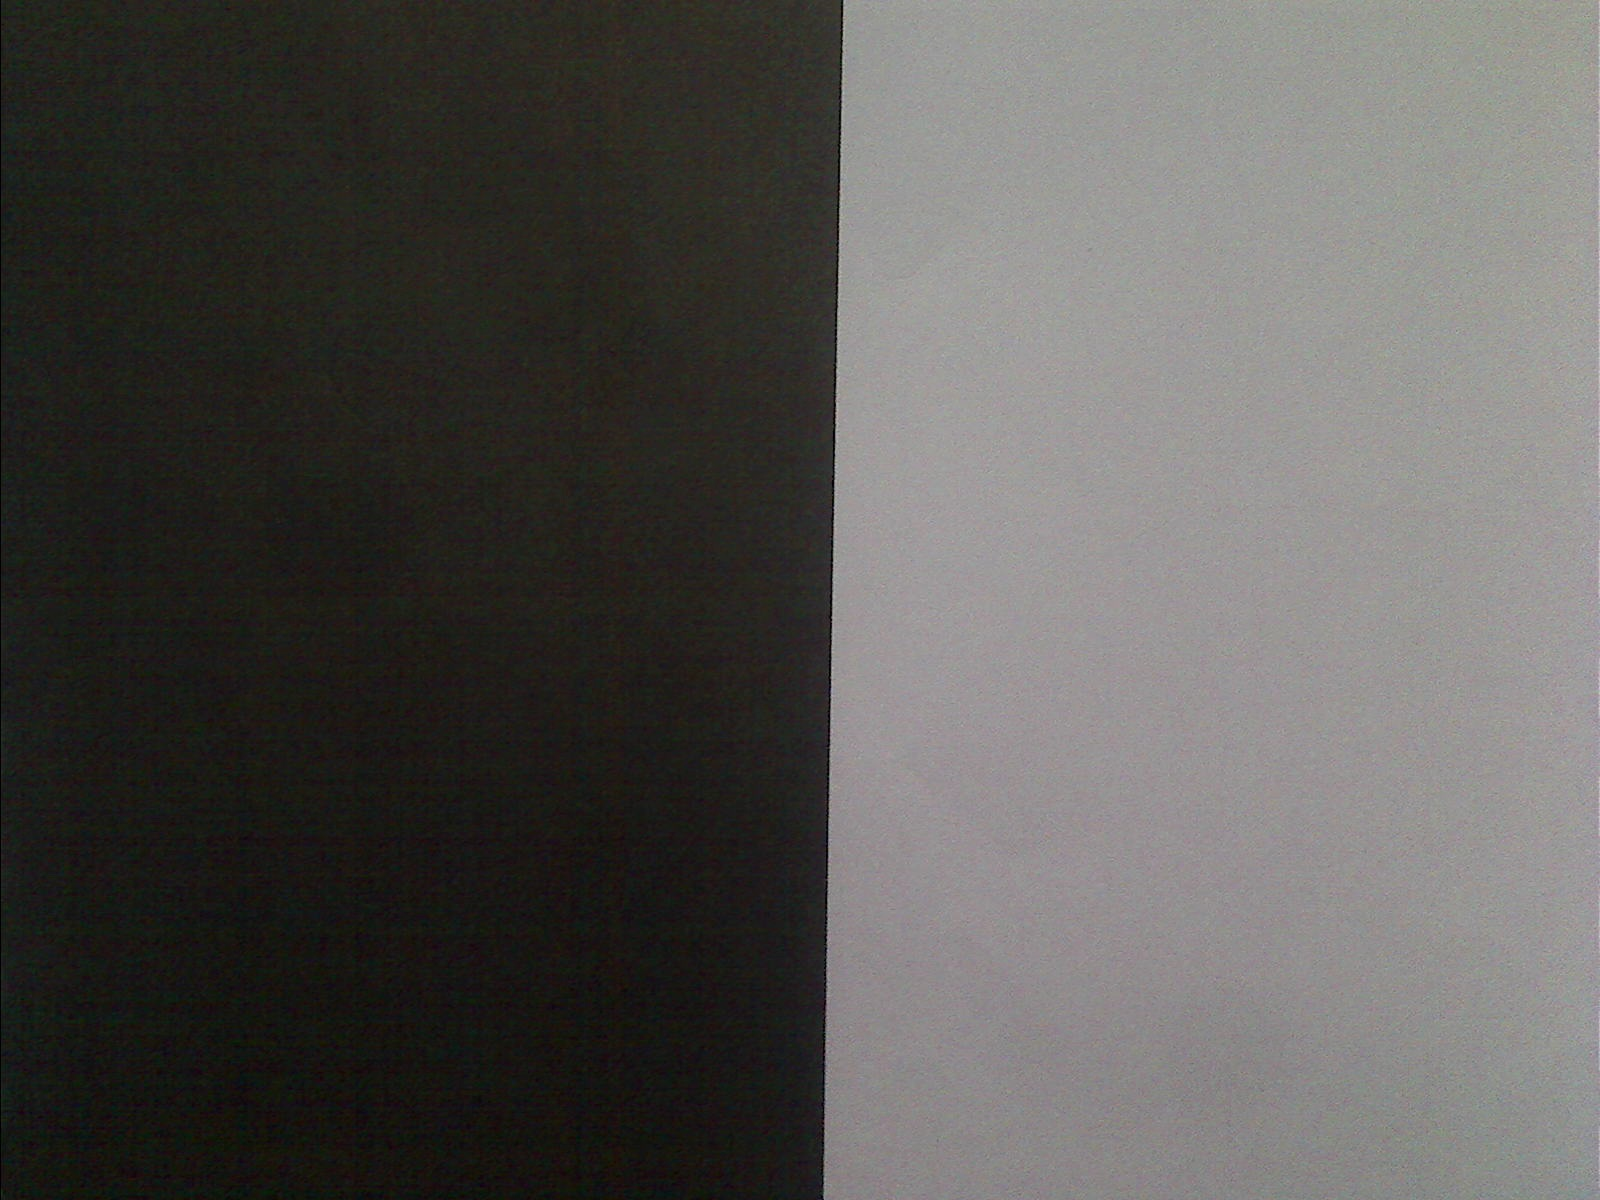
\includegraphics[width=\textwidth]{img/contrast_max_gain.jpg}
        \caption{Photo with high gain.}
    \end{subfigure}
    \caption{Photos of a step.}
\label{fig:step}
\end{figure}

\begin{figure}[H]
    \centering
    \begin{subfigure}[b]{0.47\textwidth}
        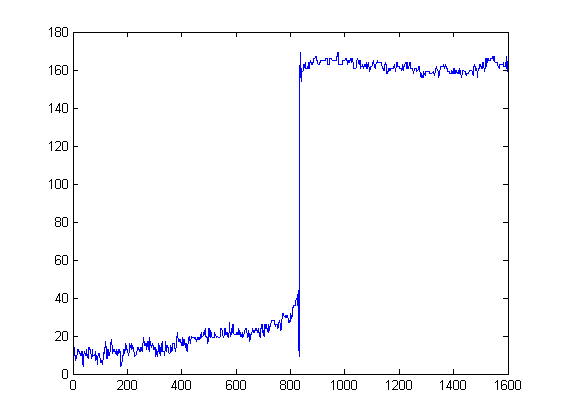
\includegraphics[width=\textwidth]{img/plot_contrast_no_gain}
        \caption{Low gain.}
    \end{subfigure}
    \begin{subfigure}[b]{0.47\textwidth}
        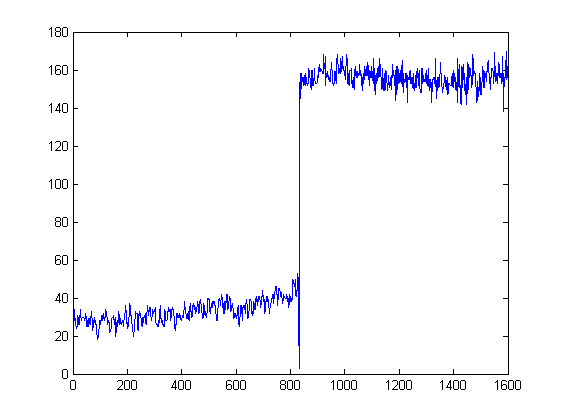
\includegraphics[width=\textwidth]{img/plot_contrast_max_gain}
        \caption{High gain.}
    \end{subfigure}
    \caption{Horizontal line plots of the red channel at $y = 600$.}
\label{fig:step_line}
\end{figure}

\begin{figure}[H]
    \centering
    \begin{subfigure}[b]{0.47\textwidth}
        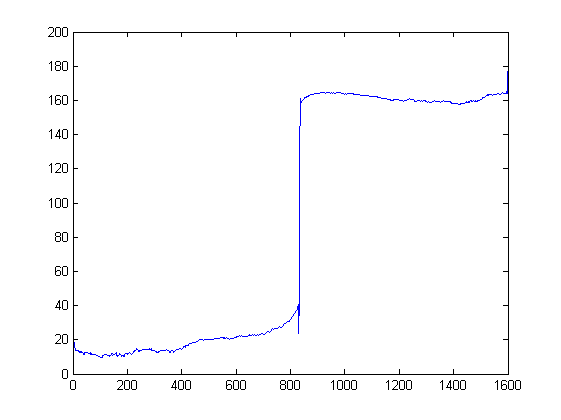
\includegraphics[width=\textwidth]{img/plot_contrast_no_gain_avg}
        \caption{Low gain.}
    \end{subfigure}
    \begin{subfigure}[b]{0.47\textwidth}
        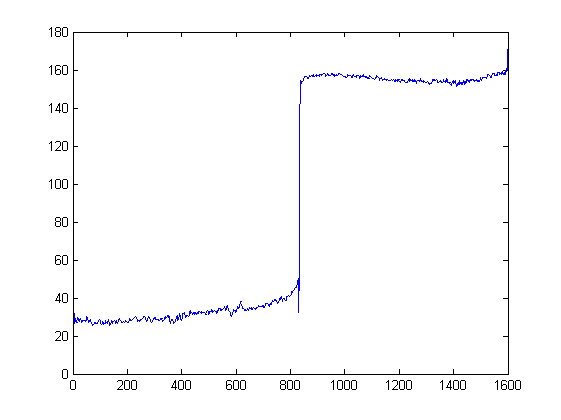
\includegraphics[width=\textwidth]{img/plot_contrast_max_gain_avg}
        \caption{High gain.}
    \end{subfigure}
    \caption{Horizontal line plots of the red channel averaged over 200 lines around $y = 600$.}
\label{fig:step}
\end{figure}

With a low gain, the average of the red column ($x=1400$) is 158.78 counts and its standard deviation is 1.85 counts.
We note that the average over 200 red columns with in the high gain image is below the average of one red column in the low gain image.
For this measure, we took the 600 first pixels of the white part of the picture.
The black part is not interesting because the vertical gradient is too high.

Therefore by its random nature, we can keep the noise low while taking a picture with high gain by averaging it over 200 columns.
To compensate the noise in high gain images – meaning that the standard deviation of the averaged columns with high gain is equal to the standard deviation of a column with low gain – the averaging over 20 columns is needed.

This method is geometric; it is limited to symmetric pictures.

\subsection{High dynamic range imaging}
% Range: x: 1200 -> 1240
%        y: 100  ->  160

% High gain: mean = 190.3185  std = 3.9500
%  low gain: mean =  63.2971  std = 0.7164

\subsubsection{Dynamic range factor}

To determine the \emph{dynamic range factor} $G$, we take two pictures of a regular surface with the same exposure time, but once with the maximal and once with the minimal gain.
Then we compare the mean value of all the pixels inside a region of interest (equation~\ref{equ:dyn_range_factor}).

\begin{figure}[H]
    \centering
    \begin{subfigure}[b]{0.47\textwidth}
        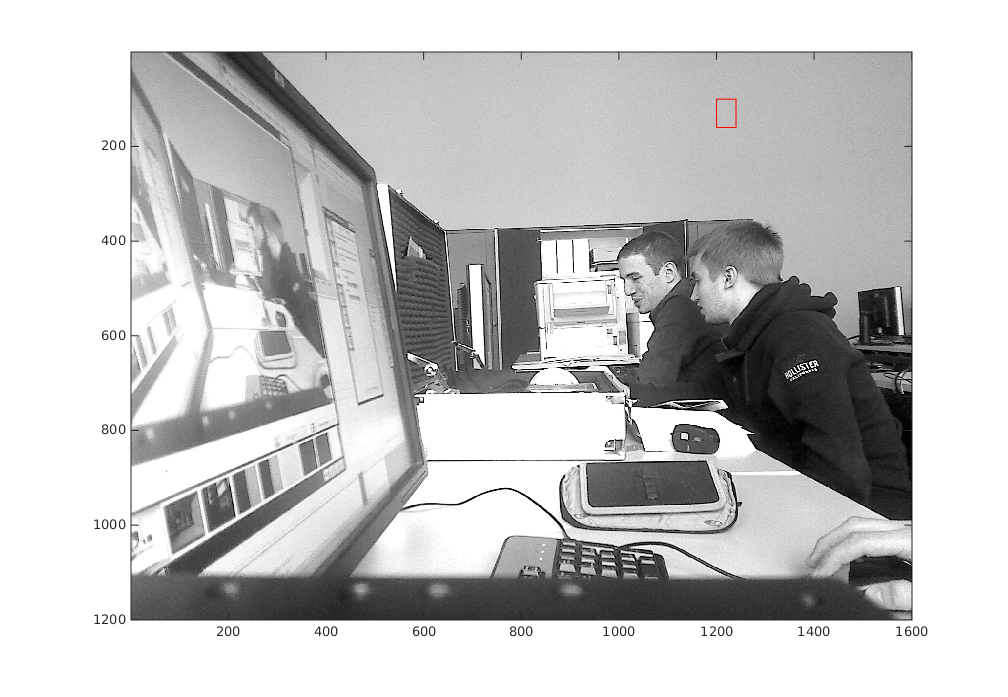
\includegraphics[width=\textwidth]{img/plot_d_range_max_gain_w_rect}
        \caption{Max gain ($\mu = 190$, $\sigma = 4.0$).}
    \end{subfigure}
    \begin{subfigure}[b]{0.47\textwidth}
        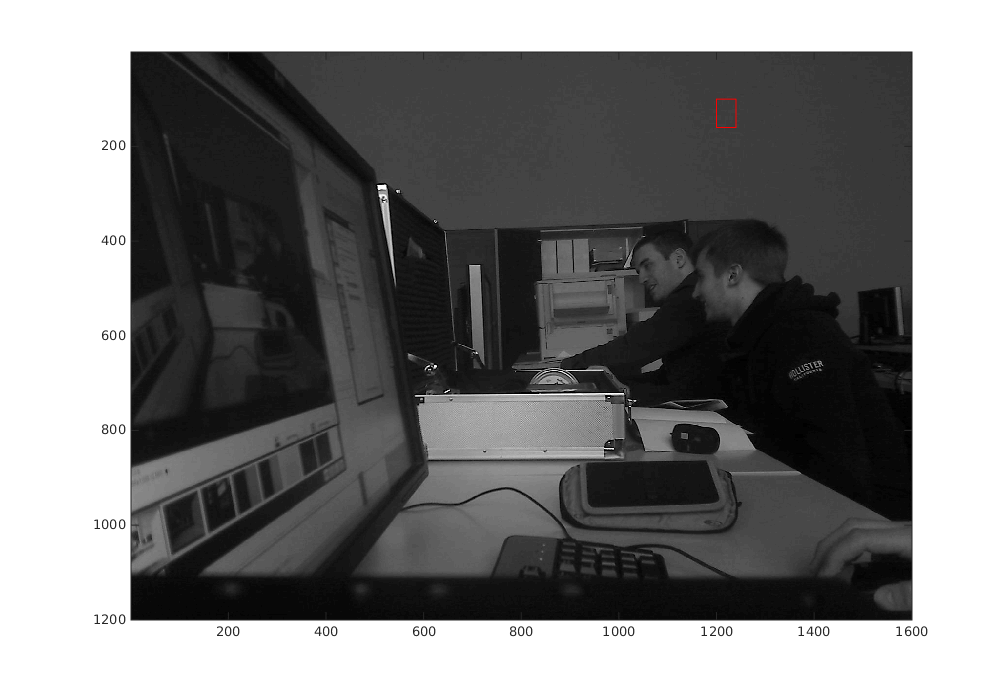
\includegraphics[width=\textwidth]{img/plot_d_range_no_gain_w_rect}
        \caption{No gain ($\mu = 63.3$, $\sigma = 0.7$).}
    \end{subfigure}
    \caption{The same image taken with different gains.
        The region of interest is marked by the red rectangle.}
\label{fig:hdr_roi}
\end{figure}

\begin{equation}
    G = \frac{\mu_H}{\mu_L} = \frac{190.32}{63.30} = 3.0
    \label{equ:dyn_range_factor}
\end{equation}

\begin{equation}
    \sigma_G = \frac{1}{\mu_L} \sigma_H + \frac{\mu_H}{\mu_L^2} \sigma_L = 0.20
    \label{equ:dyn_range_factor_err}
\end{equation}

\begin{equation}
    \frac{\Delta G}{G} = \SI{6.7}{\percent}
    \label{equ:dyn_range_factor_err_percent}
\end{equation}

We can artificially increase the dynamic range by \SI{300}{\percent}.
The error on this number of about seven percent is due to noise and a possible gradient of luminosity inside the region of interest.

\subsubsection{High dynamic range imaging example}

We take two pictures with different gains and replace the saturated pixels in the image with a high gain by the same non-saturated pixels in the low gain image (figure~\ref{fig:hdr}).

\begin{figure}[H]
    \centering
    \begin{subfigure}[b]{0.32\textwidth}
        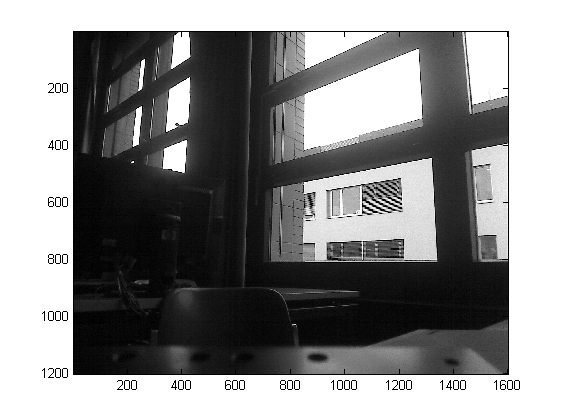
\includegraphics[width=\textwidth]{img/HDR_max_gain}
        \caption{Max gain.}
    \end{subfigure}
    \begin{subfigure}[b]{0.32\textwidth}
        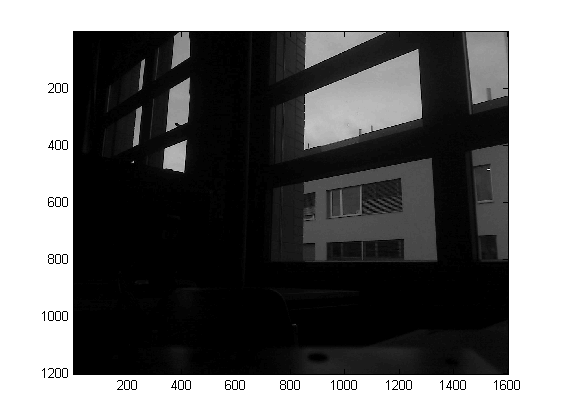
\includegraphics[width=\textwidth]{img/HDR_no_gain}
        \caption{No gain.}
    \end{subfigure}
    \begin{subfigure}[b]{0.32\textwidth}
        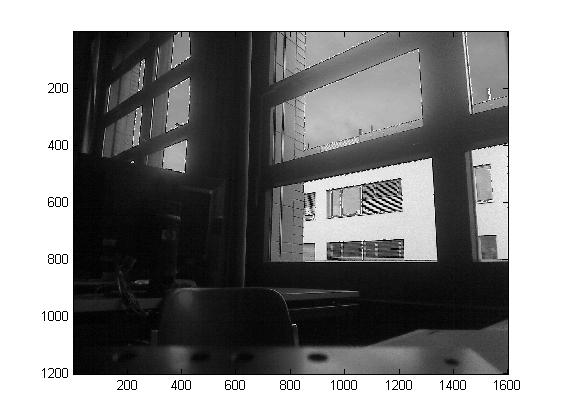
\includegraphics[width=\textwidth]{img/HDR_assembled}
        \caption{Assembled.}
    \end{subfigure}
    \caption{High dynamic range picture made by assembling two separate images with different gains.
        The borders where the two different images meet seem to be problematic.
        We speculate that this is due to a sharpness enhancement feature of the camera's software which makes the low gain image almost saturate around the borders.}
\label{fig:hdr}
\end{figure}

\subsection{Web example for HDR}

\begin{figure}[H]
    \centering
    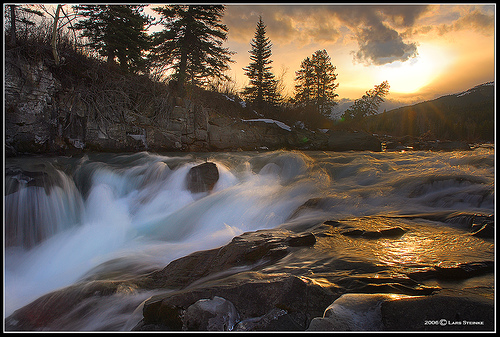
\includegraphics[width=0.8\textwidth]{img/web_example}
    \caption{We can distinguish the tree roots on the rocks and details in the clouds.
            Being able to observe these details is typical for HDR imaging.
            (Source: Larthrows on flickr)}
\label{fig:web_example}
\end{figure}

\section{Discussion and conclusions}
We saw that our measurement is limited by the \emph{dark noise} and the \emph{dynamic range}, which are both physical properties of the sensor.
The dark noise can be reduced by averaging, but this also reduces the resolution.

\emph{High dynamic range} (HDR) imaging can artificially increase the dynamic range by taking several pictures and eliminating the saturated and under-exposed parts.

\end{document}
